%%%%%%%%%%%%%%%%%%%%%%%%%%%%%%%%%%%%%%%%%%
%%%%%%%%%%%%%                 %%%%%%%%%%%%
%%%%%%%%%%%%%    EXERCISE 1   %%%%%%%%%%%%
%%%%%%%%%%%%%                 %%%%%%%%%%%%
%%%%%%%%%%%%%%%%%%%%%%%%%%%%%%%%%%%%%%%%%%
\begin{exercise}[]{
    Consider the following set of processes, with the length of the CPU burst time given in milliseconds:
    
    \begin{figure}[h]
        \begin{center}
            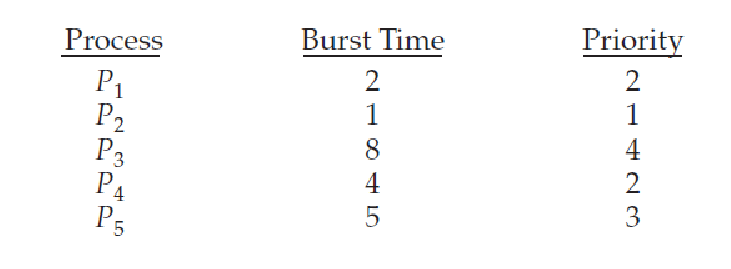
\includegraphics[scale=1]{a1.pdf}
        \end{center}
    \end{figure}

    The processes are assumed to have arrived in the order $P_1$, $P_2$, $P_3$, $P_4$, $P_5$, all at time 0.
    \begin{enumerate}
        \item [a)]
        Draw four Gantt charts that illustrate the execution of these processes using the following scheduling algorithms: FCFS, SJF, nonpreemptive priority (a larger priority number implies a higher priority), and RR (quantum = 2).
        
        \item [b)]
        What is the turnaround time of each process for each of the scheduling algorithms in part a?
        
        \item [c)]
        What is the waiting time of each process for each of these scheduling algorithms?
        
        \item [d)]
        Which of the algorithms results in the minimum average waiting time (over all processes)?
    \end{enumerate}
    }
  \begin{solution}
  \par{~}
  \begin{figure}
        \centering
        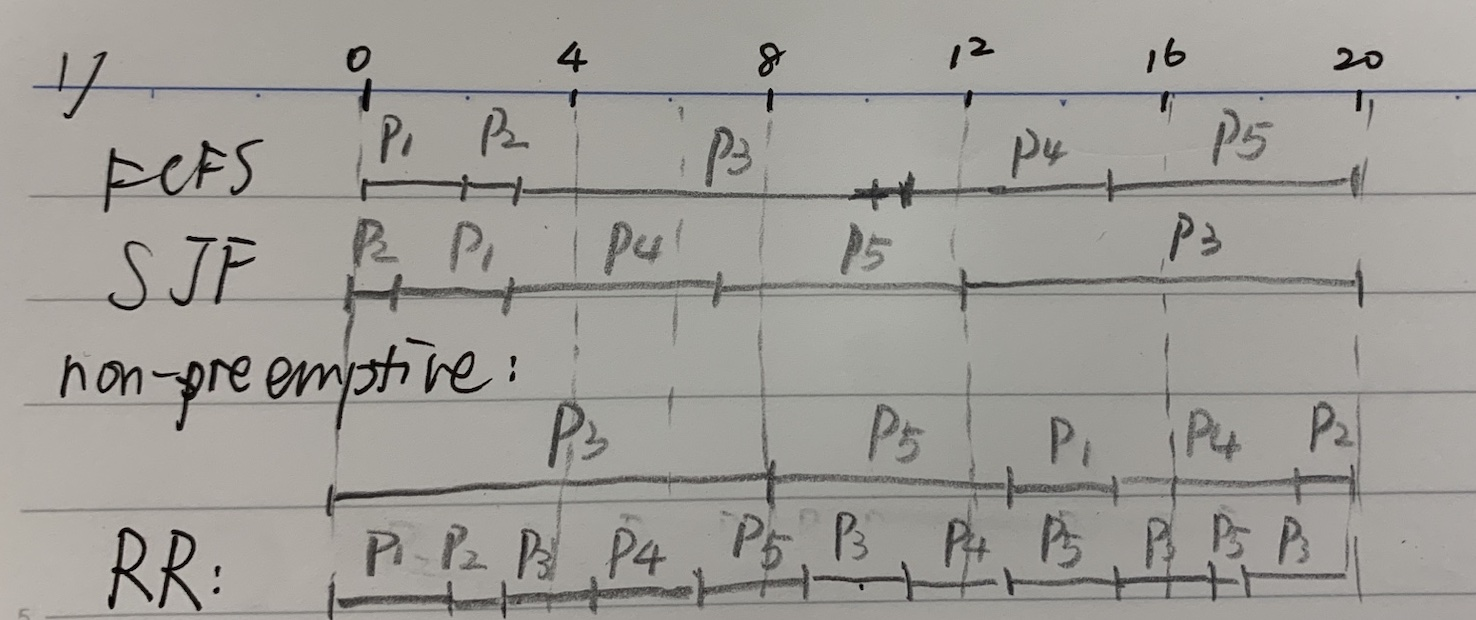
\includegraphics[width=12cm]{ex9-1.jpg}
        \caption{Exercise 1}
        \label{fig1}
    \end{figure}

    \begin{table}
        \centering
        \begin{tabular}{lccccc}
        \hline
        Turnaround Time & P1 & P2 & P3 & P4 & P5 \\ \hline
        FCFS            & 2  & 3  & 11 & 15 & 20 \\
        SJF             & 3  & 1  & 20 & 7  & 12 \\
        Non-preemptive  & 15 & 20 & 8  & 19 & 13 \\
        RR              & 2  & 3  & 20 & 13 & 18 \\ \hline
        \end{tabular}
        \caption{Exercise 1-1 \label{tab1-1}}
    \end{table}

    \begin{table}
        \centering
        \begin{tabular}{lccccc}
        \hline
        Waiting Time   & P1 & P2 & P3 & P4 & P5 \\ \hline
        FCFS           & 0  & 2  & 3  & 11 & 15 \\
        SJF            & 1  & 0  & 12 & 3  & 7  \\
        Non-preemptive & 13 & 19 & 0  & 15 & 8  \\
        RR             & 0  & 1  & 12 & 9  & 13 \\ \hline
        \end{tabular}
        \caption{Exercise 1-2 \label{tab1-2}}
    \end{table}

    \begin{table}
        \centering
        \begin{tabular}{lc}
        \hline
                       & Average Waiting Time \\ \hline
        FCFS           & 6.2                  \\
        SJF            & 4.6                  \\
        Non-preemptive & 11                   \\
        RR             & 7                    \\ \hline
        \end{tabular}
        \caption{Exercise 1-3 \label{tab1-3}}
    \end{table}
  \begin{enumerate}
      \item { See Figure \ref{fig1}. }
      \item { See Table \ref{tab1-1}. }
      \item{See Table \ref{tab1-2}. }
      \item{  See Table \ref{tab1-3}.        SJF results in minimum average waiting time.
      }
  \end{enumerate}
  \end{solution}
  \label{ex1}
\end{exercise}


%%%%%%%%%%%%%%%%%%%%%%%%%%%%%%%%%%%%%%%%%%
%%%%%%%%%%%%%                 %%%%%%%%%%%%
%%%%%%%%%%%%%    EXERCISE 2   %%%%%%%%%%%%
%%%%%%%%%%%%%                 %%%%%%%%%%%%
%%%%%%%%%%%%%%%%%%%%%%%%%%%%%%%%%%%%%%%%%%
\begin{exercise}[]{The following processes are being scheduled using a preemptive, round-robin scheduling algorithm.
    Consider the following set of processes, with the length of the CPU burst time given in milliseconds:
    \begin{figure}[h]
        \begin{center}
            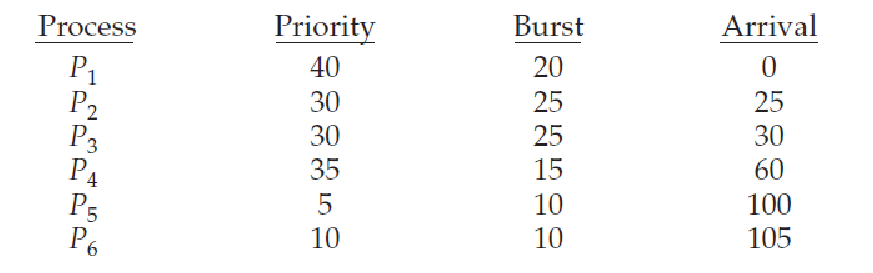
\includegraphics[scale=1]{a2.pdf}
        \end{center}
    \end{figure}
    
    Each process is assigned a numerical priority,with a higher number indicating a higher relative priority. In addition to the processes listed below, the system also has an idle task (which consumes no CPU resources and is identified as $P_{idle}$). This task has priority 0 and is scheduled whenever the system has no other available processes to run. The length of a time quantum is 10 units. If a process is preempted by a higher-priority process, the preempted process is placed at the end of the queue.
    \item [a)]
    Show the scheduling order of the processes using a Gantt chart.
    \item [b)]
    What is the turnaround time for each process?
    \item [c)]
    What is the waiting time for each process?
    \item [d)]
    What is the CPU utilization rate?
    }
  \begin{solution}
  \par{~}
  \begin{figure}
      \centering
      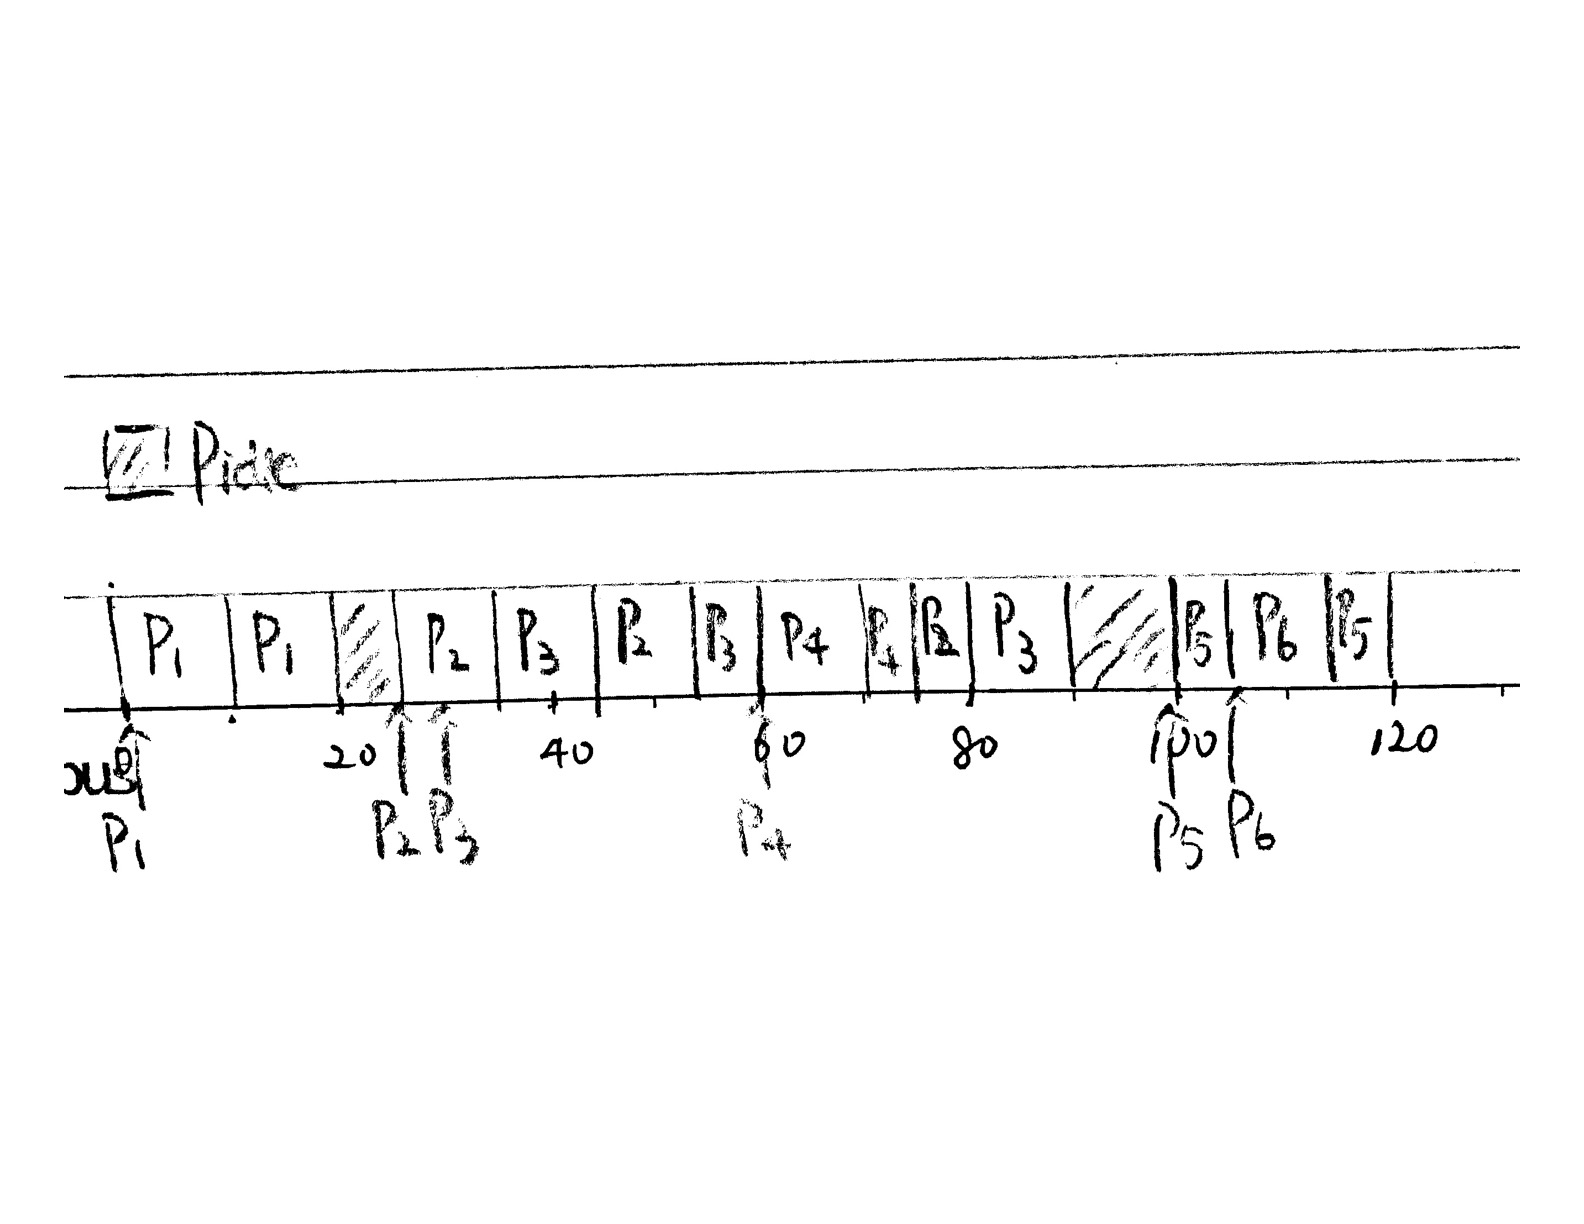
\includegraphics[width=12cm]{ex9-2.jpg}
      \caption{Exercise 2}
      \label{fig2}
  \end{figure}

  \begin{table}
      \centering
      \begin{tabular}{lllllll}
          \hline
          & P1 & P2 & P3 & P4 & P5 & P6 \\ \hline
          Turnaround Time & 20 & 55 & 60 & 15 & 20 & 10 \\
          Waiting Time    & 0  & 30 & 35 & 0  & 10 & 0  \\ \hline
      \end{tabular}
      \caption{Exercise 2\label{tab2}}
  \end{table}
  \begin{enumerate}
    \item See Figure \ref{fig2}.
    \item See Table \ref{tab2}.
    \item{
        CPU utilization rate = 105/120 = 87.5 \%
    }
    \end{enumerate}
  \end{solution}
  \label{ex2}
\end{exercise}



%%%%%%%%%%%%%%%%%%%%%%%%%%%%%%%%%%%%%%%%%%
%%%%%%%%%%%%%                 %%%%%%%%%%%%
%%%%%%%%%%%%%    EXERCISE 3   %%%%%%%%%%%%
%%%%%%%%%%%%%                 %%%%%%%%%%%%
%%%%%%%%%%%%%%%%%%%%%%%%%%%%%%%%%%%%%%%%%%
\begin{exercise}[]{The traditional UNIX scheduler enforces an inverse relationship between priority numbers and priorities: the higher the number, the lower the priority. The scheduler recalculates process priorities once per second using the following function:   
    \begin{equation} \label{apart}
        \begin{split}
        Priority = (\text{recent CPU usage} / 2) + base
        \end{split}
    \end{equation}
    where base = 60 and recent CPU usage refers to a value indicating how often a process has used the CPU since priorities were last recalculated. 
    Assume that recent CPU usage for process $P_1$ is 40, for process $P_2$ is 18, and for process $P_3$ is 10. What will be the new priorities for these three rocesses when priorities are recalculated? Based on this information, does the traditional UNIX scheduler raise or lower the relative priority of a CPU-bound process?}
  \begin{solution}
  \par{~}
  \begin{equation}
      \begin{aligned}
          Priority_1 &= 40/2+60 = 80\\
          Priority_2 &= 18/2+60 = 69\\
          Priority_3 &= 10/2+60 = 65
      \end{aligned}
  \end{equation}
  The scheduler will lower the relative priority.
  \end{solution}
  \label{ex3}
\end{exercise}